% sections/problems.tex: the section "The Problems" of the BOBILib paper, for readers
% outside the field.  It replaces Sections 2.1 and 2.2 of main.tex (from \section{Background}
% to the end of the families table); "What the Literature Had Solved" can follow it as its
% last subsection.  It keeps the labels eq:bilevel, eq:packing, fig:kip and tab:families,
% and carries sec:background as a second label, so the rest of the paper compiles unchanged.
% Counts are macros of generated/facts.tex; a count without a macro is marked "TODO macro".
% Typed numbers are instance parameters (sizes, densities, budgets, generator settings);
% each was checked against BOBILib's instance files (MPS and AUX).
% Name patterns: \pat{...} with placeholders \ph{...}; unlike \inst, a pattern may break
% before a placeholder.
\providecommand{\ph}[1]{\allowbreak\ensuremath{\langle #1\rangle}}
\providecommand{\pat}[1]{\textnormal{#1}}

\section{The Problems}\label{sec:problems}\label{sec:background}

BOBILib's \NumInstances{} instances fall into eight families (Figure~\ref{fig:familymap}). Six
are interdiction problems: a leader, the interdictor, first blocks parts of a follower's
optimization problem within a budget, and the follower then makes the best of what is left.
The other two families hold general bilevel problems, most of them built from single-level
mixed-integer linear programs (MILPs) of MIPLIB. This section describes each family: a short
story, the formal model, how BOBILib's instances are generated and named, their sizes
(Table~\ref{tab:sizes}), what makes them hard, and what was known; Table~\ref{tab:families}
anticipates the outcome of this work. The stories only illustrate the models: the instances
themselves are random, or derived from benchmark problems. In the instance names below,
\ph{n} stands for a number, for example the number of items.

\begin{figure}[t]
\centering
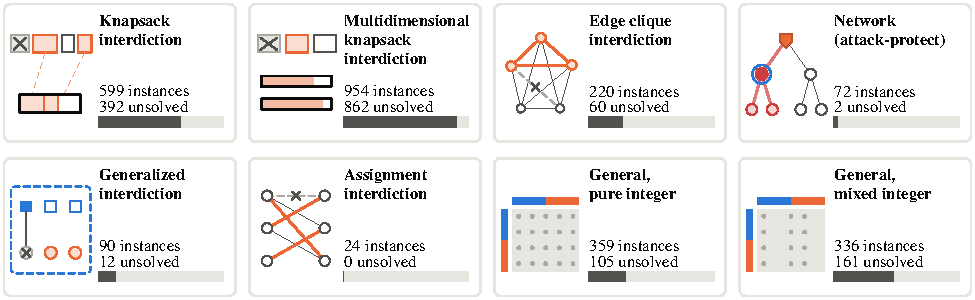
\includegraphics{figures/fig_family_map}
\caption{BOBILib at a glance: one tile per family, with its number of instances and the
number BOBILib lists as feasible or open (unsolved; the bar shows their share). In all,
\NumInstances{} instances, \NumUnsolved{} of them unsolved; BOBILib's other
\NumBobiInfeasible{} non-optimal instances are proven infeasible and all belong to the general
families.}\label{fig:familymap}
\end{figure}

\subsection{Bilevel Problems in BOBILib Form}\label{sec:prob-form}

BOBILib writes every instance with a minimizing leader:
\begin{equation}\label{eq:bilevel}
\min_{x,y}\ c\T x+d\T y\quad\text{s.t.}\quad Ax+By\ge a,\qquad
y\in\operatorname*{arg\,min}_{y'}\bigl\{f\T y' : Cx+Dy'\ge b\bigr\},
\end{equation}
with integrality requirements on some of the leader's variables $x$ and the follower's variables
$y$. For a fixed $x$ the follower solves $P(x)=\min\{f\T y: Cx+Dy\ge b\}$ (with its integrality
requirements); $x$ enters it only through the right-hand side. A point $(x,y)$ is \emph{bilevel
feasible} if it satisfies the leader's rows and integrality requirements and $y$ is optimal for
$P(x)$. When the follower has several optimal answers, the one best for the leader is assumed
(the optimistic convention, which BOBILib uses throughout). An upper-level row with a nonzero
coefficient on a follower variable is a \emph{coupling row}; a leader variable that appears in
the follower's rows is a \emph{linking variable}. The \emph{high point relaxation} (HPR) drops the
follower's optimality and keeps every row of both levels,
\[
\HPR=\min\bigl\{c\T x+d\T y : Ax+By\ge a,\ Cx+Dy\ge b,\ \text{integrality}\bigr\},
\]
so $\HPR\le\OPT$, the bilevel optimum.

Each instance is a pair of files.\cite{thurauf2026bobilib} The MPS file is the HPR: every
variable, every row of both levels, and the leader's objective. The AUX file lists the
follower's variables with their objective coefficients $f$, and the follower's rows; every
other variable and row belongs to the leader. In the interdiction families the leader's
objective and the follower's are opposite ($c=0$ and $f=-d$; for the generalized and
assignment families, see below), so the game is zero-sum, the optimistic and pessimistic
readings agree, and the model reads more naturally as $\min_x\max_y$. In most of them, each item $j$ that the
leader can block has a leader variable $x_j\in\{0,1\}$ and a follower row $x_j+y_j\le 1$
(an \emph{interdiction row}): blocking item $j$ takes it away from the follower.

\begin{table}[t]
\caption{Sizes of BOBILib's families: the sets (BOBILib's tags), the number of instances, how
many BOBILib lists as feasible or open (unsolved), and the ranges of the numbers of leader and
follower variables and rows (rows without the objective; BOBILib's metadata, checked against
the instance files). The general families contain MIPLIB models of every size.}\label{tab:sizes}
\centering\footnotesize
\setlength{\tabcolsep}{4pt}
\begin{tabular}{@{}l >{\raggedright\arraybackslash}p{1.08in} r r l r r r r@{}}
\toprule
 & & & & & \multicolumn{2}{c}{Variables} & \multicolumn{2}{c}{Rows}\\
\cmidrule(lr){6-7}\cmidrule(l){8-9}
Family & Sets & Inst. & Unsolved & Size & Leader & Follower & Leader & Follower\\
\midrule
Knapsack interdiction & \code{kp}, \code{cclw}, \code{inter-kp} & \FamKipAll & \FamKipUnsolved & 10--500 items & 10--500 & 10--500 & 1 & 11--501\\
Multidim.\ knapsack interdiction & \code{or}, \code{imkp} & \FamMkipAll & \FamMkipUnsolved & 10--500 items & 10--500 & 10--500 & 1--29 & 11--529\\
Edge clique interdiction & \code{clique}, \code{bcpins}, \code{plusbcpins} & \FamCliqueAll & \FamCliqueUnsolved & 8--60 vertices & 19--1{,}593 & 8--1{,}653 & 1 & 28--3{,}363\\
Network (attack-protect) & \code{inter-fire} & \FamNetworkAll & \FamNetworkUnsolved & 22--79 nodes & 22--79 & 44--158 & 1 & 41--974\\
Generalized interdiction & \code{generalized} & \FamGeneralizedAll & \FamGeneralizedUnsolved & $n_x,n_y\in\{20,30\}$ & 40--50 & 40--50 & 20 & 30--50\\
Assignment interdiction & \code{inter-assig} & \FamAssignmentAll & \FamAssignmentUnsolved & $5\times5$ & 25 & 25 & 1 & 45\\
General, pure integer & \code{miplib2010}, \code{miplib2017}, \code{miplib3}, \code{denegre}, \code{zhang}, \code{misc} & \FamGenPureAll & \FamGenPureUnsolved & MILPs & 1--714{,}549 & 1--714{,}549 & 0--84{,}788 & 3--169{,}576\\
General, mixed integer & \code{miplib2010}, \code{miplib2017}, \code{xuwang}, \code{xularge} & \FamGenMixedAll & \FamGenMixedUnsolved & MILPs & 10--399{,}808 & 10--399{,}808 & 0--480{,}585 & 4--961{,}170\\
\bottomrule
\end{tabular}
\end{table}

\begin{table}[t]
\caption{BOBILib's families and the outcome for the instances it lists as feasible or open.
Published: optimal in published work (for \NumLitNoFile{} of them only the published value is
used; Section~\ref{sec:verify}). Here: proven optimal in this work. No point: no bilevel feasible
point exists. New point: a verified bilevel feasible point where BOBILib lists none (for
\NumPointPublishedBefore{} of them a point had been published; Section~\ref{sec:res-overview}).
The total includes BOBILib's \FamAssignmentAll{} assignment interdiction instances, which it lists
as optimal.}\label{tab:families}
\centering\small
\begin{tabular}{@{}l r r r r r r r@{}}
\toprule
 & & Feasible & \multicolumn{5}{c}{Outcome for the feasible or open instances}\\
\cmidrule(l){4-8}
Family & Instances & or open & Published & Here & No point & New point & Unchanged\\
\midrule
Knapsack interdiction (KIP) & \FamKipAll & \FamKipUnsolved & \FamKipLit & \FamKipNew & \FamKipNoFeas & \FamKipFirst & \FamKipUnchanged\\
Multidim.\ knapsack interdiction (MKIP) & \FamMkipAll & \FamMkipUnsolved & \FamMkipLit$^{\dagger}$ & \FamMkipNew & \FamMkipNoFeas & \FamMkipFirst & \FamMkipUnchanged\\
Edge clique interdiction & \FamCliqueAll & \FamCliqueUnsolved & \FamCliqueLit & \FamCliqueNew & \FamCliqueNoFeas & \FamCliqueFirst & \FamCliqueUnchanged\\
Network interdiction & \FamNetworkAll & \FamNetworkUnsolved & \FamNetworkLit & \FamNetworkNew & \FamNetworkNoFeas & \FamNetworkFirst & \FamNetworkUnchanged\\
Generalized interdiction & \FamGeneralizedAll & \FamGeneralizedUnsolved & \FamGeneralizedLit & \FamGeneralizedNew & \FamGeneralizedNoFeas & \FamGeneralizedFirst & \FamGeneralizedUnchanged\\
General, pure integer & \FamGenPureAll & \FamGenPureUnsolved & \FamGenPureLit & \FamGenPureNew & \FamGenPureNoFeas & \FamGenPureFirst & \FamGenPureUnchanged\\
General, mixed integer & \FamGenMixedAll & \FamGenMixedUnsolved & \FamGenMixedLit & \FamGenMixedNew & \FamGenMixedNoFeas & \FamGenMixedFirst & \FamGenMixedUnchanged\\
\midrule
Total & \NumInstances & \NumUnsolved & \NumLitOptimal & \NumNewOptimal & \NumNoFeasible & \NumFirstPoint & \NumUnchanged\\
\bottomrule
\multicolumn{8}{@{}l}{\footnotesize $^{\dagger}$Includes \inst{\OrClosureName}, whose published lower bound is
inconsistent but whose published branch-and-cut bound closes it (Section~\ref{sec:res-or}).}
\end{tabular}
\end{table}

% --------------------------------------------------------------------------------------
\subsection{Knapsack Interdiction}\label{sec:prob-kip}

\textbf{The story.} A smuggler fills a container of limited capacity with the most valuable
goods it can get. Before that, an inspector, with a limited budget of inspection hours, bans
some of the goods; each ban costs hours. The inspector wants the smuggler's best load to be
worth as little as possible. The inspector is the leader and the smuggler the follower.

\textbf{The model.} This is a packing interdiction problem. Items are $N=\{1,\dots,n\}$. The
leader chooses $x\in\{0,1\}^n$ within budget rows $Gx\le g$, and the follower packs what is
left:
\begin{equation}\label{eq:packing}
\Phi(x)=\max\bigl\{p\T y : Wy\le c,\ y\le \mathbf{1}-x,\ y\in\{0,1\}^n\bigr\},\qquad
\OPT=\min\bigl\{\Phi(x): Gx\le g,\ x\in\{0,1\}^n\bigr\},
\end{equation}
with nonnegative integer profits $p$, weights $W$ and capacities $c$ (from here on, $c$ denotes
capacities, not the cost vector of~\eqref{eq:bilevel}). The knapsack interdiction problem (KIP)
has one leader row, $a\T x\le\beta$ with costs $a$ and budget $\beta$, and one follower row,
$w\T y\le c$ with weights $w$ and capacity $c$; the multidimensional KIP (MKIP,
Section~\ref{sec:prob-mkip}) has several of either. In BOBILib form the leader minimizes $p\T y$
and the follower minimizes $-p\T y$. In the files the rows are the budget, the capacity and the
$n$ interdiction rows $x_j+y_j\le 1$, so an instance with $n$ items has $2n$ variables and $n+2$
rows. In the \emph{subset-sum class} each item's profit equals its weight ($p=w$), so the
follower's value is the largest sum of surviving weights that fits the capacity.
Figure~\ref{fig:kip} shows a small instance.

\begin{figure}[t]
\centering
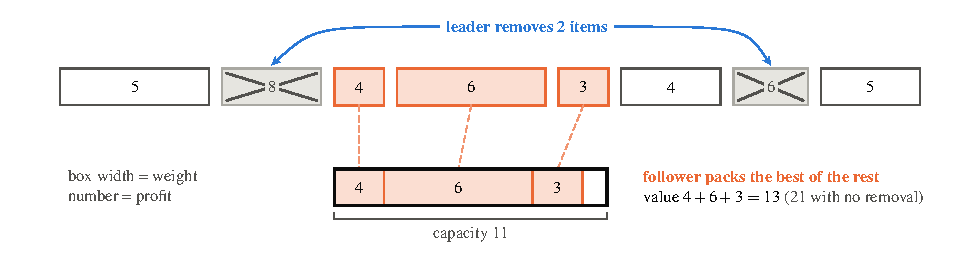
\includegraphics{figures/fig_knapsack_interdiction}
\caption{Knapsack interdiction on a toy instance (box width = weight, number = profit). The
leader removes two items, and the follower packs the best of what is left into its knapsack.
The removal shown cuts the follower's best packing from 21 to 13, and no other pair of removals
does as well.}\label{fig:kip}
\end{figure}

\textbf{The instances.} BOBILib has three KIP sets.
\begin{itemize}\setlength{\emergencystretch}{3em}
\item \code{kp} (450 instances; % TODO macro
Fischetti, Monaci and Sinnl\cite{fischetti2018dynamic}), named
\pat{interKP-\ph{n}-\ph{R}-\ph{t}-\ph{I}}, for example \inst{interKP-200-100-6-3}: $n\in\{100,200,\dots,500\}$
items, coefficient range $R=100$, item class $t\in\{1,\dots,9\}$ and instance number
$I\in\{1,\dots,10\}$. The follower's weights and profits come from the knapsack generator of
Martello, Pisinger and Toth\cite{martello1999dynamic} in class $t$: 1~uncorrelated, 2~weakly
correlated, 3~strongly correlated, 4~inverse strongly correlated, 5~almost strongly correlated,
6~subset sum ($p=w$), 7~even-odd subset sum ($p=w$, even weights), 8~even-odd strongly
correlated, 9~uncorrelated with similar weights. The instance number sets the capacity,
$c=\lfloor I\sum_j w_j/11\rfloor$ (in classes 7 and 8 raised to the next odd number when even),
so it grows from about 9\% to 91\% of the total weight. The leader's costs are integers between
0 and $R$, and its budget $\beta$ lies within 10 of $c$. In class~9 the budget exceeds the sum of
all leader costs, so the leader can block every item; Fischetti et al.\ left these instances out
as trivial, BOBILib keeps them.
\item \code{cclw} (50 instances; % TODO macro
Caprara, Carvalho, Lodi and Woeginger\cite{caprara2016bilevel}), named
\pat{interdiction\ph{n}-\ph{I}}: the same construction with uncorrelated items, $n\in\{35,40,\dots,55\}$.
\item \code{inter-kp} (99 instances; % TODO macro
DeNegre\cite{denegre2011thesis}), named \pat{K50\ph{n}W\ph{i}.KNP}: $n\in\{10,20,\dots,50\}$ items,
instance $i\in\{1,\dots,20\}$ (\inst{K5010W01} is missing), built from bicriteria knapsack
instances, whose first objective gives the follower's profits and whose second gives the
leader's costs; the budget is half the total cost, rounded up.
\end{itemize}

\textbf{What makes it hard.} The follower's problem alone, one knapsack with at most 500 items,
is easy in practice. The difficulty is the leader's: it chooses among exponentially many subsets,
and the follower's value $\Phi(x)$ jumps as $x$ changes, with no convexity to exploit. Already
this two-level knapsack problem is $\Sigma_2^p$-complete.\cite{caprara2014complexity} The HPR,
the starting point of general bilevel solvers, is worthless here: it lets the follower pack
nothing ($y=0$), so its value is 0. The subset-sum classes are hard in another way: the follower
can usually fill its knapsack exactly, so the optimum is often the trivial bound $c$ (or $c-1$ in
class~7, where every sum of weights is even and $c$ is odd), as in all \NumNewKip{} instances
the literature left open, and a proof must show that no leader choice within the budget prevents
a fill that close.

\textbf{What was known.} BOBILib lists \FamKipUnsolved{} KIP instances as not optimal.
Weninger and Fukasawa's combinatorial branch and bound\cite{weninger2025fast} solves
\NumLitKip{} of them; the \NumNewKip{} it leaves open, all in classes~6 and~7 with 200 or more
items, are solved in Section~\ref{sec:kip}.

% --------------------------------------------------------------------------------------
\subsection{Multidimensional Knapsack Interdiction}\label{sec:prob-mkip}

\textbf{The story.} The smuggler's container now has a weight limit and a volume limit, and each
good uses some of both; the inspector's budget may also have several parts (hours of different
teams). Blocking the most valuable goods is no longer the obvious move: what matters is which
goods let the smuggler use both limits well (Figure~\ref{fig:mkip}).

\textbf{The model.} Model~\eqref{eq:packing} with several rows in $G$ (the leader's budgets) or
in $W$ (the follower's knapsacks), or both. In BOBILib's MKIP instances every row, the leader's
and the follower's alike, is a row of one multidimensional knapsack problem (MKP) with $K$ rows:
the follower packs items within its rows, and the leader blocks items within its rows, paying for
a block what the item would weigh in those rows.

\begin{figure}[t]
\centering
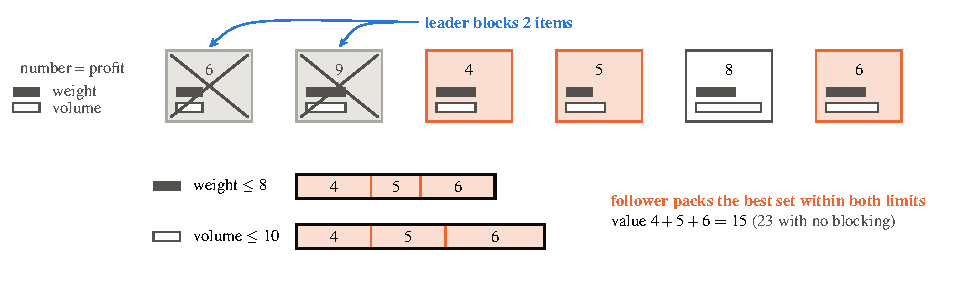
\includegraphics{figures/fig_mkip}
\caption{Multidimensional knapsack interdiction on a toy instance: every item has a profit, a
weight and a volume, and the follower's knapsack has a limit for each. The leader blocks two
items; the follower then packs the most valuable set that fits both limits (value 15 instead of
23). Blocking the two most valuable items (9 and 8) would leave 17.}\label{fig:mkip}
\end{figure}

\textbf{The instances.} Both sets come from Fischetti, Ljubi\'c, Monaci and
Sinnl.\cite{fischetti2019interdiction} Each MKP gives three instances, which differ only in how
its $K$ rows are split; the suffix \code{-0}, \code{-50} or \code{-100} names the split. In
variant \code{-0} the leader has the first row and the follower the other $K-1$; in variant
\code{-50} the leader has the first $\lceil K/2\rceil$ rows and the follower the rest; in variant
\code{-100} the leader has all rows but the last, so the follower has a single knapsack.
\begin{itemize}\setlength{\emergencystretch}{3em}
\item \code{or} (\NumOr{} instances), named \pat{OR\ph{K}x\ph{n}-\ph{\alpha}\_\ph{i}.dat-\ph{v}}, for example
\inst{OR10x100-0.25\_1.dat-50}: built on Chu and Beasley's MKPs from the OR-Library (Operations
Research Library),\cite{chu1998genetic,beasley1990orlibrary} with $n\in\{100,250,500\}$ items,
$K\in\{5,10,30\}$ rows, tightness $\alpha\in\{0.25,0.5,0.75\}$ and ten instances $i$ for each
combination. The weights are integers between 0 and 1,000; an item's profit is, up to
rounding, its average weight over the $K$ rows plus a random amount between 0 and 500. The right-hand side of every row, the
leader's budget rows and the follower's capacity rows alike, is $\alpha$ times the sum of its
coefficients, rounded to an integer (below, ``budget 25\%'' means $\alpha=0.25$). So variant
\code{-100} has one follower knapsack, and variants \code{-0} and \code{-50} have several.
\item \code{imkp} (\NumImkp{} instances), named after the MKP with the same suffixes, for example
\inst{weish26.dat-50}: built on the SAC-94 suite\cite{khuri1994zero} (the instances
\inst{hp}, \inst{pb}, \inst{pet}, \inst{sento}, \inst{weing} and \inst{weish}), with 10 to 105
items and 2 to 30 rows. When $K=2$ the three splits coincide, and only variant \code{-50} is kept.
\end{itemize}

\textbf{What makes it hard.} Everything that makes KIP hard, and more. The follower's problem is
now a multidimensional knapsack: a dynamic program would need a state for every combination of
used capacities, and the linear programming (LP) relaxation, on which most bounds rest, can
overestimate the follower's value by up to the profit of one item per follower row
(Theorem~\ref{thm:bracket}). The largest OR instances have 500 items and 30 rows.

\textbf{What was known.} Fischetti et al.\ solved all \NumImkp{} imkp instances, but BOBILib lists
\NumLitImkp{} of them as only feasible. No OR instance is optimal in BOBILib; Lozano, Bergman and
Cire\cite{lozano2026network} proved \NumLitOr{} optimal and published bounds for most of the
others.

% --------------------------------------------------------------------------------------
\subsection{Edge Clique Interdiction}\label{sec:prob-clique}

\textbf{The story.} In a communication or social network, a clique, a group in which everyone is
linked to everyone else, is a tightly knit cluster; large ones shorten the paths along which
information travels.\cite{furini2021branch} The leader can cut up to $k$ links and wants the largest cluster
that survives to be as small as possible; the follower, after the cuts, finds the largest
cluster left.

\textbf{The model.} The graph $G=(V,E)$ has $n=|V|$ vertices and $m=|E|$ edges. The leader deletes
a set $D$ of at most $k$ edges, and the follower's value is the clique number $\omega(G-D)$, the
size of a largest clique of the remaining graph. BOBILib's \code{clique} instances write the
follower's problem with a variable $y^V_v$ per vertex and $y^E_e$ per edge, and the leader's with
$x_e$ per edge:\cite{fischetti2018dynamic,tang2016class}
\[
\min_{x\in\{0,1\}^E}\Bigl\{\max\textstyle\sum_{v\in V}y^V_v :
y^V_u+y^V_v\le 1\ (\{u,v\}\notin E),\
y^V_u+y^V_v-y^E_{uv}\le 1,\ x_{uv}+y^E_{uv}\le 1\ (\{u,v\}\in E)\Bigr\}
\quad\text{s.t.}\ \textstyle\sum_{e\in E}x_e\le k,
\]
with binary $y$. An edge the leader deletes cannot be used ($y^E_e=0$), and two vertices that are
not joined by a usable edge cannot both be in the clique. So a \code{clique} instance has $m$
leader variables, $n+m$ follower variables, one leader row and $n(n-1)/2+m$ follower rows.
Figure~\ref{fig:clique} (Section~\ref{sec:clique}) shows a small instance.

\textbf{The instances.}
\begin{itemize}\setlength{\emergencystretch}{3em}
\item \code{clique} (\NumCliqueSet{} instances; Fischetti, Monaci and Sinnl\cite{fischetti2018dynamic}),
named \pat{normalClique\ph{n}-\ph{100d}-\ph{i}}, for example \inst{normalClique60-70-2}: random graphs with
$n\in\{40,50,60\}$ vertices and edge density $d\in\{0.7,0.9\}$, that is
$m=\lfloor d\,n(n-1)/2\rfloor$ edges chosen at random, budget $k=\lfloor m/4\rfloor$, and ten
graphs $i$ for each $n$ and $d$.
\item \code{bcpins} and \code{plusbcpins} (Tang, Richard and Smith\cite{tang2016class}; Fischetti
et al.\cite{fischetti2018dynamic}), named \pat{BCPIns\_\ph{n}\_\ph{10d}\_\ph{i}.txt\_trad.txt\_K\ph{k}} and
\pat{plusBCPIns\_\ph{n}\_\ph{10d}\_\ph{i}}: smaller random graphs, $n\in\{8,10,12,15\}$, the same densities,
budget $k=\lceil m/4\rceil$ and ten graphs for each $n$ and $d$. The \code{bcpins} files use a
compact follower model with vertex variables only, one row per pair of vertices; the
\code{plusbcpins} files use the model above, strengthened by extra valid
inequalities.\cite{fischetti2018dynamic} BOBILib lists all of them as optimal.
\end{itemize}

\textbf{What makes it hard.} Finding a maximum clique is NP-hard, and the follower's formulation
is weak: setting every $y^V_v=1/2$ and every $y^E_e=0$ satisfies all its rows, so its LP
relaxation is worth at least $n/2$, 20 to 30 here, while every value BOBILib lists is at most
\CliqueBobiMax. The leader picks $k$ of $m$ edges, for example \CliqueKSixtySeven{} of
\CliqueMSixtySeven{}, and a general solver must close the gap between the weak relaxation and the
true value by branching over these choices. As for knapsack interdiction, the HPR is worth 0.

\textbf{What was known.} BOBILib lists all \NumCliqueSet{} \code{clique} instances as feasible, with
values \CliqueBobiMin{} to \CliqueBobiMax; Fischetti et al.\ used them to test heuristics, and no
optimum had been published. Section~\ref{sec:clique} proves \NumNewClique{} of them optimal.

% --------------------------------------------------------------------------------------
\subsection{Network Interdiction: The Attack-Protect Game}\label{sec:prob-network}

\textbf{The story.} A fire, a computer virus or a rumor starts at some nodes of a network and
spreads along its links. An attacker, the leader, chooses up to $\Phi$ nodes to set on fire. A
defender, the follower, then protects up to $\Lambda$ nodes. The fire spreads from the attacked
nodes to every neighbor that is not protected, and from there on; a node is saved if the fire
never reaches it. The defender maximizes the number of saved nodes and the attacker minimizes
it (Figure~\ref{fig:network}, Section~\ref{sec:network}). (Here $\Phi$ is a budget, as in BOBILib's
row names, not the value function of~\eqref{eq:packing}.)

\textbf{The model.} The instances come from the multilevel critical node problem of Baggio,
Carvalho, Lodi and Tramontani,\cite{baggio2021multilevel} a three-level game in which a defender
first vaccinates $\Omega$ nodes, the attacker then attacks and the defender then protects.
BOBILib keeps the last two levels, the attack-protect game, on the graph without the vaccinated
nodes, as used by Fischetti et al.\cite{fischetti2017new} With $x_v=1$ for an attacked node,
$z_v=1$ for a protected node and $s_v=1$ for a saved node (all binary),
\[
\min_{x}\Bigl\{\max_{z,s}\textstyle\sum_v s_v :
\sum_v z_v\le\Lambda,\ s_v+x_v\le 1\ (v\in V),\
s_u\le s_v+z_u\ (\text{every edge }\{u,v\}\text{, both directions})\Bigr\}
\quad\text{s.t.}\ \textstyle\sum_v x_v\le\Phi.
\]
An attacked node is not saved, and a node that is not protected is saved only if all its
neighbors are. So an instance on $n'$ nodes and $e'$ edges has $n'$ leader variables, $2n'$
follower variables, one leader row and $n'+2e'+1$ follower rows. (In the files the attack
variables are named \code{y}, the protections \code{x} and the saved nodes \code{a}.)

\textbf{The instances.} The set \code{inter-fire} has \FamNetworkAll{} instances. Their names,
such as \inst{tree-50\_1-5-5\_006}, have the form
\pat{\ph{G}-\ph{n}\_\ph{\Omega}-\ph{\Phi}-\ph{\Lambda}\_\ph{i}}: graph type
$G$ (\code{tree}, a random tree grown one node at a time, or \code{rndgraph}, a random graph of a
given density), $n\in\{25,50,80\}$ nodes before vaccination, the three budgets, and the instance
number. Each file has $n'=n-\Omega$ nodes, and its rows \code{Phi} and \code{Lambda} have the
budgets of the name (checked for all \FamNetworkAll{} files).

\textbf{What makes it hard.} The follower's best protection depends on the whole shape of the
attack, and the leader has many attacks to choose from: \NetworkAttacks{} sets of at most
\NetworkPhi{} of \NetworkNodes{} nodes in the two unsolved instances. Again the HPR, in which
the follower may save nothing, is worth 0.

\textbf{What was known.} BOBILib lists \NetworkBobiOptimal{} of the \FamNetworkAll{} instances as
optimal; the other \FamNetworkUnsolved{}, two trees with \NetworkNodes{} nodes and
$\Phi=\Lambda=\NetworkPhi$, are solved in Section~\ref{sec:network}.

% --------------------------------------------------------------------------------------
\subsection{Generalized Interdiction}\label{sec:prob-generalized}

\textbf{The story.} The leader now has its own plans and constraints. Think of a regulator that
chooses projects to fund; funding some of them rules out a matching activity of a firm. The
firm, the follower, then chooses its activities to maximize its own profit, and the regulator's
cost and constraints depend on what the firm does. Unlike in the families above, the two
objectives are not opposite.

\textbf{The model.} Fischetti, Monaci and Sinnl's generalized interdiction
problem\cite{fischetti2018dynamic} (Figure~\ref{fig:generalized}) is
\[
\min_{x,y}\ c_x\T x+c_y\T y\quad\text{s.t.}\quad G_xx+G_yy\le G_0,\quad
y\in\operatorname*{arg\,max}_{y'}\bigl\{d\T y' : By'\le b,\ y'_j\le 1-x_j\ (j\in N),\ y'\ge 0,\
\text{integrality}\bigr\},
\]
with binary leader variables. The set $N$ pairs some leader variables with follower variables:
$x_j=1$ forbids $y_j$. The leader's rows contain the follower's variables (they are coupling
rows), so the follower's answer can violate them; the follower's rows contain no leader
variables except in the interdiction rows.

\textbf{The instances.} The set \code{generalized} has \FamGeneralizedAll{} random
instances,\cite{fischetti2018dynamic} named \pat{general\ph{n_x}-\ph{n_y}-\ph{|N|}-20-20-\ph{i}}, for example
\inst{general20-30-20-20-20-2}: $n_x\in\{20,30\}$ binary leader variables, $n_y\in\{20,30\}$ binary
follower variables, $|N|\in\{10,20,30\}$ interdiction pairs ($|N|\le\min\{n_x,n_y\}$), 20 leader
rows and 20 follower rows, and ten instances for each allowed combination. The coefficients are
random integers between $-50$ and $50$. Each leader row has a binary slack variable that costs the
leader 100,000, and each follower row a continuous slack variable that costs the follower 100,000,
so every row can always be satisfied, at a price. With the slacks and the interdiction rows, an
instance has $n_x+20$ leader variables, $n_y+20$ follower variables, 20 leader rows and $20+|N|$
follower rows.

\textbf{What makes it hard.} The game is not zero-sum, so methods built for interdiction do not
apply, and because of the coupling rows the follower's optimal answer can push the leader into
paying for slack. The penalties also make objective values large next to coefficients of at most
50; in \inst{general20-30-20-20-20-2} the follower's optimum at BOBILib's leader choice is
\GenTolPhiOpt, and at that scale a relative tolerance hides absolute errors of many units
(Section~\ref{sec:discussion}).

\textbf{What was known.} BOBILib lists \FamGeneralizedUnsolved{} of the \FamGeneralizedAll{}
instances as feasible and the rest as optimal; Lozano, Bergman and Cire\cite{lozano2026network}
proved \NumLitGeneralized{} of the \FamGeneralizedUnsolved{} optimal.

% --------------------------------------------------------------------------------------
\subsection{Assignment Interdiction}\label{sec:prob-assignment}

\textbf{The story and the model.} A dispatcher, the follower, assigns 5 workers to 5 jobs, one
job each, at the least total cost. Beforehand the leader, within a budget, forbids some
worker-job pairs, to make the dispatcher's cheapest assignment as expensive as possible
(Figure~\ref{fig:assignment}). The follower has a binary variable per pair, 20 rows that give
every worker exactly one job and every job exactly one worker, and 25 interdiction rows; the
leader has one budget row.

\textbf{The instances.} The set \code{inter-assig} has \FamAssignmentAll{} instances,
\inst{2AP05-1} to \inst{2AP05-25} without \inst{2AP05-12}, which BOBILib left out as invalid. DeNegre
built them from bicriteria assignment problems:\cite{denegre2011thesis} the first objective is
the follower's cost, the second gives the leader's costs in the budget row. In 19 of the files % TODO macro
the leader's objective is exactly the negated follower cost; in the other five it differs. % TODO macro
BOBILib lists all of them as optimal, and this work does not consider them further.

\begin{figure}[t]
\centering
\begin{minipage}[b]{0.47\textwidth}
\centering
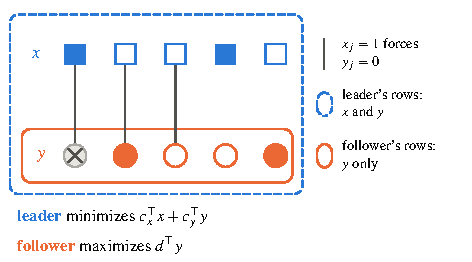
\includegraphics{figures/fig_generalized}
\end{minipage}\hfill
\begin{minipage}[b]{0.47\textwidth}
\centering
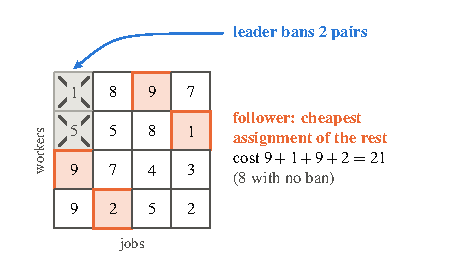
\includegraphics{figures/fig_assignment}
\end{minipage}\par\vspace{4pt}
\begin{minipage}[t]{0.47\textwidth}
\caption{Generalized interdiction: the leader's variables $x$ and the follower's $y$; for the
interdiction pairs, $x_j=1$ forces $y_j=0$. The leader's rows contain $x$ and $y$, the
follower's only $y$, and the two objectives differ.}\label{fig:generalized}
\end{minipage}\hfill
\begin{minipage}[t]{0.47\textwidth}
\caption{Assignment interdiction on a toy instance (row = worker, column = job, number = cost).
The leader bans two pairs; the follower's cheapest assignment of the rest costs 21 instead of
8.}\label{fig:assignment}
\end{minipage}
\end{figure}

% --------------------------------------------------------------------------------------
\subsection{General Instances from MIPLIB and Other MILPs}\label{sec:prob-general}

\textbf{The story.} Take a real planning model, say a schedule, a network design or a
production plan, stored as a MILP in MIPLIB, the library of benchmark MILPs.
Hand half of its decisions to a second party, who decides after the first and works against
it. The first party, the leader, now has to plan for the worst reply of the second.

\textbf{The construction.} A MILP $\min\{c\T z: \text{rows},\ \text{integrality}\}$ with $n$
variables and $m$ rows becomes a bilevel instance by splitting its variables and rows between the
two levels and giving the follower an objective (Figure~\ref{fig:miplib}). BOBILib has three
constructions; the following was checked on every one of its % TODO macro: 389
MIPLIB-derived instances.
\begin{itemize}\setlength{\emergencystretch}{3em}
\item \code{miplib2010} and \code{miplib2017} (Kleinert and Schmidt;\cite{kleinert2021computing}
from MIPLIB~2010 and MIPLIB~2017\cite{koch2011miplib,gleixner2021miplib}), named after the MILP
with a suffix: the leader gets the first $\lceil n/2\rceil$ variables in the order of the file,
and the follower the rest. In \pat{\ph{X}\_0\_100} all rows are the follower's (0\% at the leader,
100\% at the follower); in \pat{\ph{X}\_50\_50} the first $\lceil m/2\rceil$ rows are the leader's
and the rest the follower's. In all but two of the \inst{\_50\_50} instances some leader row % TODO macro
contains follower variables, so they have coupling rows; the \inst{\_0\_100} instances have none.
The third variant, with every row at the leader, leaves the follower without rows and so
without linking variables; BOBILib excludes such instances, as it excludes MILPs that are
infeasible or have range rows or a zero follower objective, and MIPLIB~2017 models already in
MIPLIB~2010.\cite{thurauf2026bobilib}
\item \code{miplib3} (Fischetti et al.;\cite{fischetti2016intersection,fischetti2018intersection}
from MIPLIB~3,\cite{bixby1998miplib} 20 binary models, three instances each), % TODO macro
named \pat{\ph{X}-\ph{k}} with $k\in\{0.100000,0.500000,0.900000\}$, for example \inst{air03-0.100000}:
the follower gets the first $\lfloor kn\rfloor$ variables and the leader the rest; all rows are
the follower's, so the leader has no rows at all.
\end{itemize}
In all three the leader keeps the MILP's objective $c$ on all variables, and the follower
minimizes $-c$ on its own variables (in the AUX files of 90 instances these coefficients are % TODO macro
rounded to six significant digits, for example 83.2776 for $-c_j=83.2776042$ in
\inst{gen-ip002\_0\_100}). So for a fixed leader choice the follower makes the leader's cost on
its variables as high as it can, and the HPR is the original MILP. BOBILib calls an instance
\emph{mixed integer} if it has at least one continuous and one integer variable, and \emph{pure
integer} otherwise.

\begin{figure}[t]
\centering
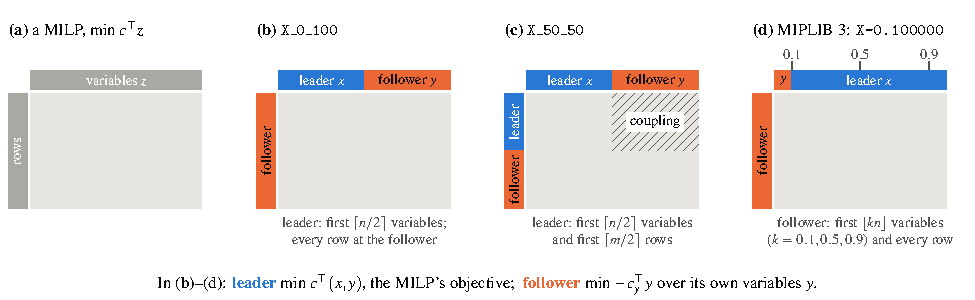
\includegraphics{figures/fig_miplib_split}
\caption{How BOBILib turns a MILP (a) into a bilevel instance. (b)~\pat{\ph{X}\_0\_100}: the leader
gets the first half of the variables, the follower the rest and every row. (c)~\pat{\ph{X}\_50\_50}:
the leader also gets the first half of the rows, which then contain follower variables (coupling
rows). (d)~MIPLIB~3 instances \pat{\ph{X}-\ph{k}}: the follower gets the first fraction $k$ of the
variables and every row. The leader keeps the MILP's objective; the follower minimizes its
negation on its own variables.}\label{fig:miplib}
\end{figure}

\textbf{The other general sets.} The other general instances are random or small: \code{denegre}
(110 random pure integer instances made with DeNegre's generator,\cite{denegre2011thesis} % TODO macro
50 of them from his thesis), \code{zhang} % TODO macro
(30 pure integer instances of {\"O}zaltin and Zhang\cite{ozaltin2017branch}), \code{misc} (6 small % TODO macro
examples from the literature, among them two of Moore and Bard\cite{moore1990mixed}),
\code{xuwang} (100 mixed integer instances of Xu and Wang,\cite{xu2014exact} with 10 to 460 % TODO macro
variables per level) and \code{xularge} (60 larger ones, 500 to 1,000 variables per level, built % TODO macro
the same way by Fischetti et al.\cite{fischetti2017new}). BOBILib lists all of them as optimal
except one in \code{misc}, \inst{milp\_10\_20\_50\_2310}, which is feasible. % TODO macro: one

\textbf{What makes them hard.} The HPR alone is a MIPLIB model, and some of these are hard MILPs
in their own right; the largest bilevel instances have hundreds of thousands of variables and
rows (Table~\ref{tab:sizes}). Checking a single point requires solving the follower's MILP to
optimality. Linking variables can be continuous, which BOBILib's two solvers do not handle
(Section~\ref{sec:general}); all 137 instances with continuous linking variables are % TODO macro
MIPLIB-derived and unsolved in BOBILib. In \inst{\_50\_50} instances the coupling rows can make the
follower's best answer infeasible for the leader; and in some instances the follower's problem
is infeasible or unbounded for every leader choice, so no bilevel feasible point exists at all
(Section~\ref{sec:general}).

\textbf{What was known.} Almost all of the \NumGeneralUnsolved{} unsolved general instances are
MIPLIB-derived. Their statuses come from BOBILib's one-hour solver runs, and published work had
solved \NumLitMiplib{} of them (Section~\ref{sec:general} and the next subsection).
